\clearpage

\section{Applying RISE}
\nblink{nhs-chest-xray/analyze/rise.ipynb}
\nblink{nhs-chest-xray/analyze/rise\_bounding\_boxes.ipynb}

The implementation of RISE on the NIH Chest X-ray dataset with the DenseNet model was straightforward, because the reference implementation of RISE on GitHub \cite{risegithub} already contains a working implementation for PyTorch. The implementation was not published on the Python Packaging Index, so the code had to be downloaded and added into our GitHub repository.

\subsection{Results}

\begin{figure}[H]
    \centering
    \begin{subfigure}[t]{.45\textwidth}
        \centering
        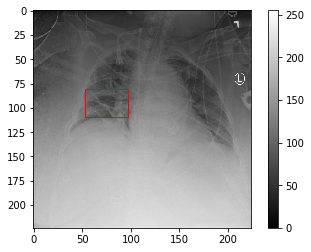
\includegraphics[width=\linewidth]{chapters/03_classification/images/rise0_bbox.png}
        \caption{Original image with bounding box added by a physician}
    \end{subfigure}\hspace{1cm}%
    \begin{subfigure}[t]{.45\textwidth}
        \centering
        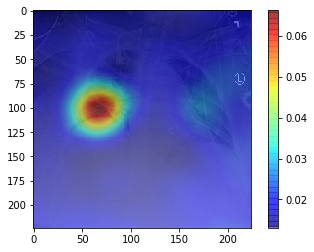
\includegraphics[width=\linewidth]{chapters/03_classification/images/rise0_saliency.png}
        \caption{RISE saliency map of (a)}
    \end{subfigure}
    \caption{Image (a) shows the input image with the bounding box added by the physician, showing which region is relevant for the diagnosis. Image (b) is a RISE saliency map which shows that the neural network considers the same region of the image as relevant for the correct classification.}
    \label{rise_example_1}
\end{figure}

\begin{figure}[H]
    \centering
    \begin{subfigure}[t]{.45\textwidth}
        \centering
        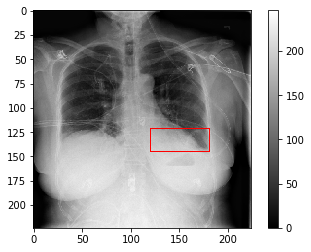
\includegraphics[width=\linewidth]{chapters/03_classification/images/rise1_bbox.png}
        \caption{Original image with bounding box added by a physician}
    \end{subfigure}\hspace{1cm}%
    \begin{subfigure}[t]{.45\textwidth}
        \centering
        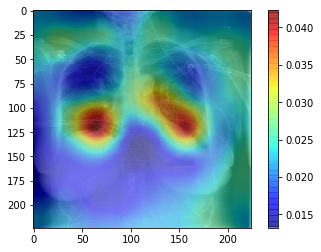
\includegraphics[width=\linewidth]{chapters/03_classification/images/rise1_saliency.png}
        \caption{RISE saliency map of (a)}
    \end{subfigure}
    \caption{Image (a) shows the input image with the bounding box added by the physician, showing which region is relevant for the diagnosis. Image (b) is a RISE heat map which highlights multiple regions that are important for the correct classification of this image.}
    \label{rise_example_2}
\end{figure}

\begin{figure}[H]
    \centering
    \begin{subfigure}[t]{.45\textwidth}
        \centering
        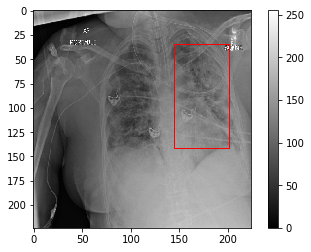
\includegraphics[width=\linewidth]{chapters/03_classification/images/rise2_bbox.png}
        \caption{Original image with bounding box added by a physician}
    \end{subfigure}\hspace{1cm}%
    \begin{subfigure}[t]{.45\textwidth}
        \centering
        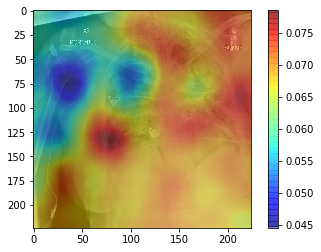
\includegraphics[width=\linewidth]{chapters/03_classification/images/rise2_saliency.png}
        \caption{RISE saliency map of (a)}
    \end{subfigure}
    \caption{Image (a) shows the input image with the bounding box added by the physician. Image (b) is a RISE heat map which highlights many regions which should be completely irrelevant for the classification. The classification is still correct.}
    \label{rise_example_3}
\end{figure}



\subsection{Discussion}
Figure \ref{rise_example_1} shows that the bounding box created by the physician perfectly matches the region the neural network uses to generate the correct classification. In comparison, in Figure \ref{rise_example_2} the RISE heat map shows two regions which the neural network considers import for the correct classification. In this case, consultation with a physician is required if looking at those two places is correct for the diagnosis or if the neural network is wrong.

As a last example, Figure \ref{rise_example_3} shows a heat map where regions are highlighted that should have no influence at all at a correct diagnosis. All three generated heat maps for this class Infiltration look similar, and are therefore an indicator that physicians can not depend on the correct diagnosis for this class.

Most heat maps look similar to the ones in Figure \ref{rise_example_2}, showing more regions relevant for the classification than the bounding boxes. This discrepancy have to be checked with a physician can not easily be dismissed as an error by the neural network.

\subsection{Conclusion}
The generated heat maps by RISE allow a good and accurate insight into the inner working of the neural network. It clearly showed in which cases the network could not be trusted and in which cases the classifications where made based on the correct image region.
